\assignementTitle{Музыкальный AR-интерфейс}{20}{4}

Команда AltFuture разрабатывает вместе с коллегами из Японии музыкальный интерфейс в дополненной реальности для разного вида шоу и выставок. На Андрея, ведущего 3D-дизайнера компании, возложили проектировку трехмерных моделей музыкальных инструментов для AR-интерфейса. В ходе работы над проектом, Андрей заметил, что на чертеже одного из музыкальных инструментов,  коллегами из Японии указаны размры не всех объектов. На рисунке показан эскиз модели, присланный иностранными специалистами.

\begin{figure}[h]
    \begin{minipage}[h]{0.49\linewidth}
    \center{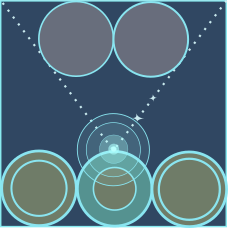
\includegraphics[width=1\linewidth]{1.png} \\ а) Ожидаемый результат }
    \end{minipage}
    \hfill
    \begin{minipage}[h]{0.49\linewidth}
    \center{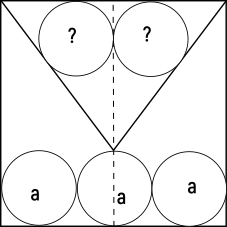
\includegraphics[width=1 \linewidth]{2.png} \\ б) Макет}
    \end{minipage}
    
\end{figure}

На чертеже изображен квадрат, на нижней стороне которого располагаются 3 круга одного размера. Треугольником обозначено, как будет идти волна распространения звука в игре. Видно, что одно из соударений волны проходит через центр квадрата, задевая среднюю окружность. А вот размер двух окружностей, который оказались вписанными в треугольник остались неизвестны. 
Андрей предположил, что размеры всех 5 окружностей, равны и решил делать модель с расчетом на это. Докожите, что предположение Андрея верно.\\